\section{Main Screen}
\begin{figure}[H]
    \centering
    \includegraphics[width=0.4\textwidth]{images/MainScreen2.png}
    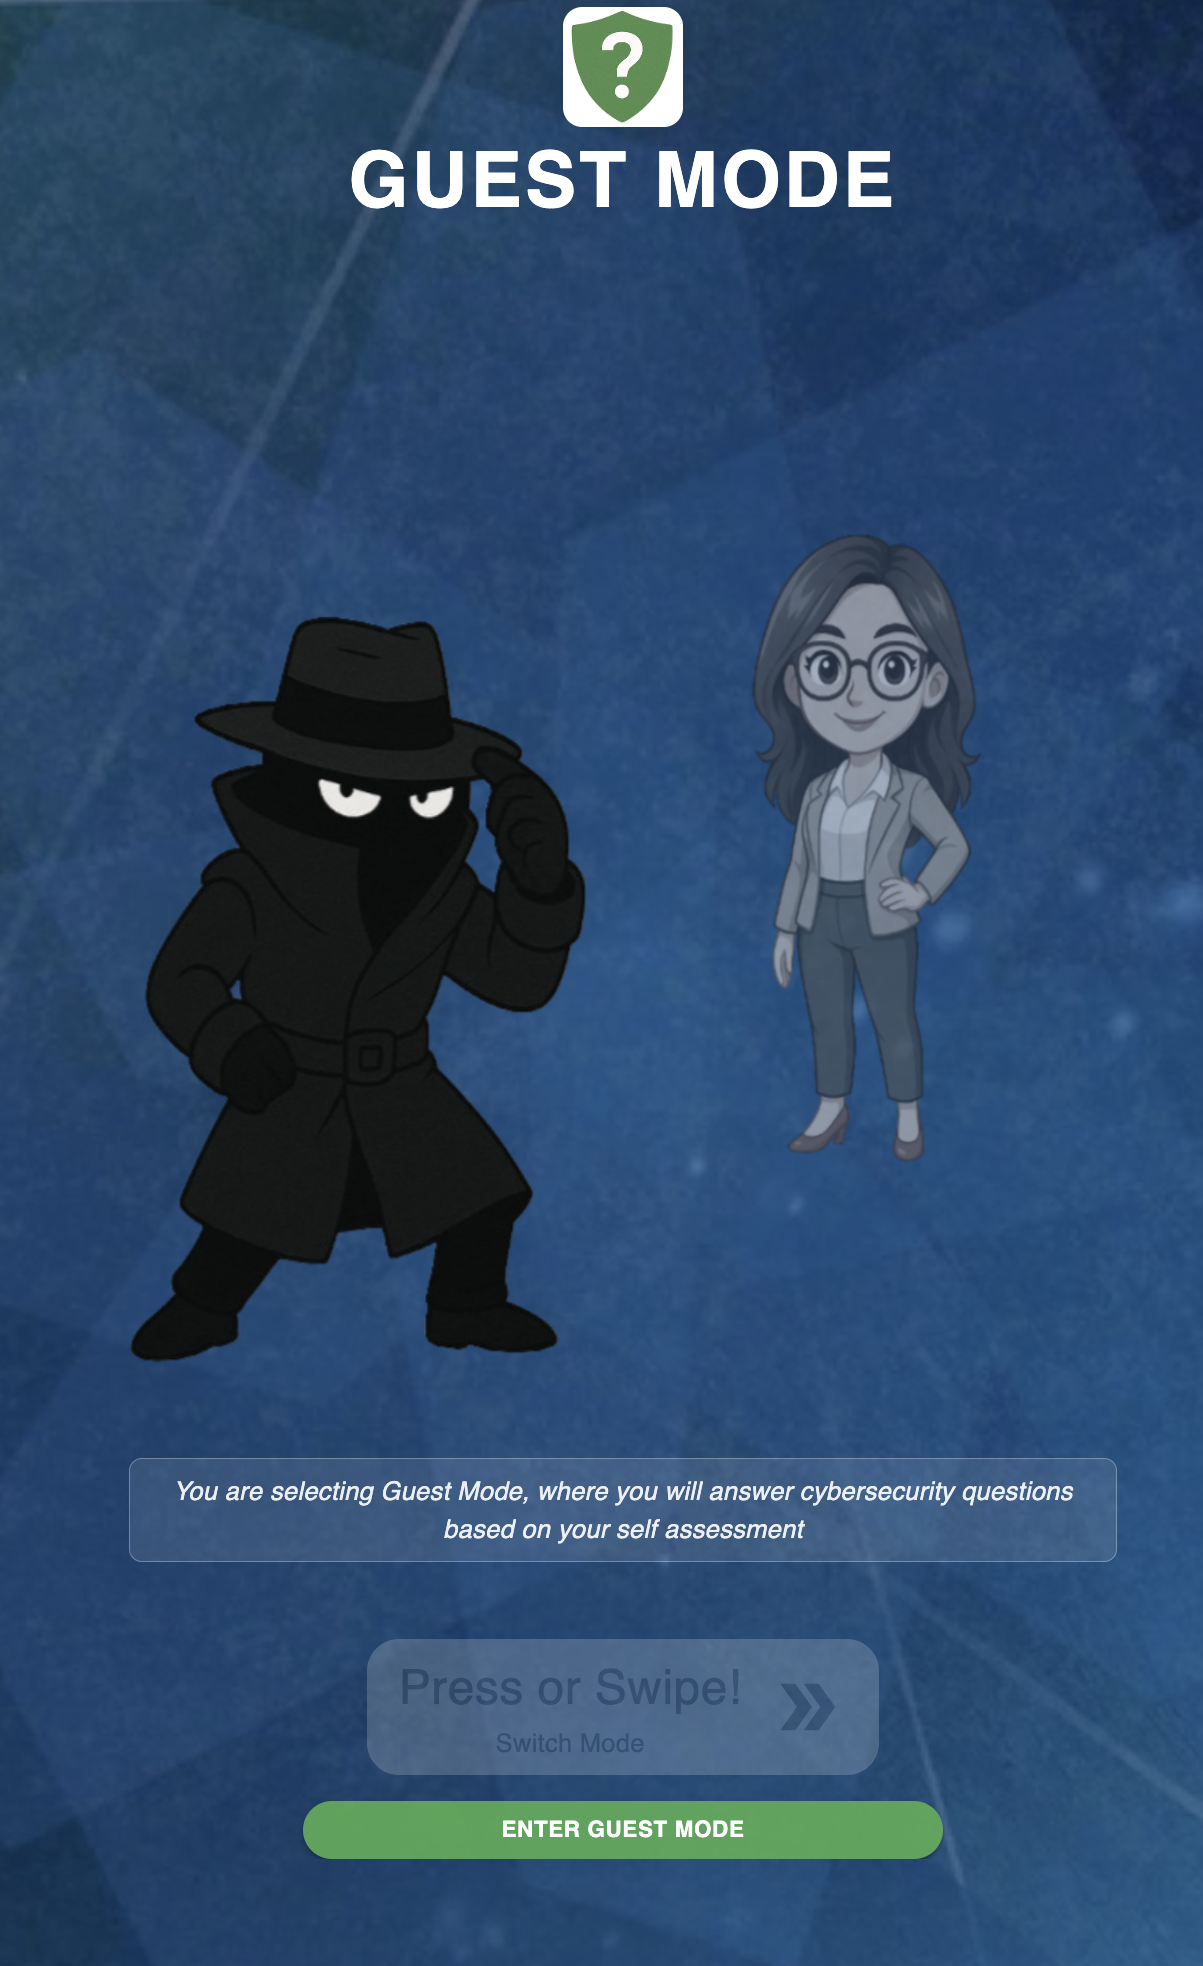
\includegraphics[width=0.4\textwidth]{images/MainScreenCharacters.png}
    \caption{Main Screen (Left) Characters for Mode selection (Right)}
\end{figure}

When the system is offline, the display shows a static screen where \textbf{security tips and news} 
are dynamically fetched by the LLM. These messages are designed to catch users’ attention and encourage 
them to engage with \textbf{SeQG} and learn more about \textbf{cybersecurity}.
When a user approaches the display and taps the screen, two mode characters appear, each accompanied 
by a short explanation of their functionality.